\documentclass[12pt,a4paper]{article}

%-----------------------------------
% Packages
%-----------------------------------
\usepackage[utf8]{inputenc}
\usepackage[english]{babel}
\usepackage{graphicx}
\usepackage{float}
\usepackage{geometry}
\usepackage{booktabs}
\usepackage{longtable}
\usepackage{hyperref}
\usepackage{enumitem}
\usepackage{array}
\usepackage{listings}
\usepackage{xcolor}
\usepackage{caption}
\usepackage{subcaption}
\usepackage{multicol}
\usepackage{tabularx}

\geometry{
    left=2.5cm,
    right=2.5cm,
    top=2.5cm,
    bottom=2.5cm
}

\hypersetup{
    colorlinks=true,
    linkcolor=blue,
    citecolor=blue,
    urlcolor=blue
}

\lstset{
    basicstyle=\ttfamily\small,
    backgroundcolor=\color{gray!10},
    frame=single,
    breaklines=true,
    columns=fullflexible
}

\title{
ETL Health Colombia --- ODS 3:\\
Dimensional Data Warehouse for\\
Healthcare Analytics
}

\author{
Deyton Riascos Ortiz --- Project Manager\\
Samuel Izquierdo Bonilla --- Development Team\\
Daniel David Garcia Restrepo --- Product Owner\\
Mauricio Taborda Gongora --- Tester
}

\date{September 16, 2026}

\begin{document}

\maketitle

\tableofcontents

\newpage

%%%%%%%%%%%%%%%%%%%%%%%%%%%%%%%%%%%%%%
\section{Introduction}

\subsection{Problem Definition}

Colombia's healthcare system (SGSSS) faces significant territorial disparities in access to services. While the country has achieved high affiliation rates nationally, the distribution of healthcare infrastructure (beds, procedural rooms, equipment) does not proportionally match the population's needs across departments and municipalities. Some regions maintain high capacity per affiliate while others face critical shortages.

This project builds a dimensional data warehouse that integrates two complementary datasets from the Colombian Ministry of Health:

\begin{enumerate}[nosep]
    \item \textbf{Affiliates (SISPRO):} Number of healthcare affiliates by department, municipality, and regime type (Subsidized, Contributory, Special, Individual).
    \item \textbf{Facilities (REPS):} Installed healthcare infrastructure capacity (beds, rooms, equipment) by facility, department, and municipality.
\end{enumerate}

Understanding the relationship between affiliation density and infrastructure capacity is essential for identifying underserved regions and informing resource allocation decisions.

\subsection{SDG Alignment}

This project is aligned with \textbf{UN Sustainable Development Goal 3 --- Good Health and Well-Being}, specifically \textbf{Target 3.8: Achieve universal health coverage (UHC)}, including financial risk protection, access to quality essential healthcare services, and access to safe, effective, quality, and affordable essential medicines and vaccines for all.

The analysis directly addresses Target 3.8 by examining:
\begin{itemize}[nosep]
    \item \textbf{Coverage breadth} (R1, R2): Measuring how many Colombians are affiliated and where they are located.
    \item \textbf{Service availability} (R3, R4): Assessing whether healthcare infrastructure exists to serve the affiliated population.
    \item \textbf{Equity} (R5): Examining whether access is equitably distributed across regimes and territories.
\end{itemize}

\subsection{Geographic and Population Scope}

\begin{itemize}[nosep]
    \item \textbf{Geographic scope:} National --- 33 departments + Bogot\'{a} D.C., across all municipalities.
    \item \textbf{Population of interest:} Affiliates of the Colombian healthcare system and healthcare facilities (IPS).
    \item \textbf{Potential stakeholders:} Ministry of Health and Social Protection (Minsalud), departmental health secretaries, EPS (healthcare promoting entities), hospital managers, healthcare policy researchers.
\end{itemize}

%%%%%%%%%%%%%%%%%%%%%%%%%%%%%%%%%%%%%%
\section{Analytical Objectives and Requirements}

\subsection{Analytical Objective}

Analyze the distribution of healthcare affiliates and infrastructure capacity across Colombian territories to identify geographic disparities and support resource allocation decisions aligned with SDG Target 3.8.

\subsection{Requirements Matrix (R1--R5)}

\begin{table}[H]
\centering
\small
\begin{tabularx}{\textwidth}{p{1cm} X X X}
\toprule
\textbf{ID} & \textbf{Analytical Requirement} & \textbf{Business Question} & \textbf{Decision Supported}\\
\midrule
R1 & Determine the total number of affiliates by regime type nationally & How many Colombians are affiliated to each regime (Subsidized, Contributory, Special, Individual)? & Understand the composition of the healthcare system for policy planning.\\
\addlinespace
R2 & Identify the departments with the highest and lowest affiliate density & Which departments concentrate the most/least affiliates? & Detect territorial disparities to prioritize interventions.\\
\addlinespace
R3 & Analyze the distribution of healthcare facilities by nature (public/private) and care level & What is the public-private mix and at what care levels? & Evaluate whether the private sector complements public infrastructure.\\
\addlinespace
R4 & Compare installed capacity per affiliate across departments & Which departments have sufficient infrastructure relative to their affiliated population? & Identify regions where expansion is needed.\\
\addlinespace
R5 & Assess the relationship between regime type and geographic distribution & Are Subsidized affiliates concentrated in different territories than Contributory? & Understand whether regime segmentation maps to geographic inequity.\\
\bottomrule
\end{tabularx}
\caption{Analytical requirements matrix.}
\end{table}

%%%%%%%%%%%%%%%%%%%%%%%%%%%%%%%%%%%%%%
\section{Data Sources}

\subsection{Source Selection}

\begin{table}[H]
\centering
\small
\begin{tabularx}{\textwidth}{p{3cm} X X}
\toprule
\textbf{Characteristic} & \textbf{Affiliates Dataset} & \textbf{Facilities Dataset}\\
\midrule
Source & SISPRO --- Sistema Integrado de Informaci\'{o}n de la Protecci\'{o}n Social & REPS --- Registro Especial de Prestadores de Servicios de Salud\\
Owner & Ministerio de Salud y Protecci\'{o}n Social & Ministerio de Salud y Protecci\'{o}n Social\\
URL & datos.gov.co & datos.gov.co\\
Format & CSV (period as thousand separator) & CSV\\
Records & 3,369 rows & 41,427 rows (9,320 unique facilities)\\
Attributes & 8 columns & 20 columns\\
Temporal & April 2022 (Q2 snapshot) & November 2022 (Q4 snapshot)\\
Measures & \texttt{NumPersonas} (affiliates) & \texttt{num cantidad capacidad instalada} (capacity)\\
\bottomrule
\end{tabularx}
\caption{Data source characteristics.}
\end{table}

\subsection{Dataset Suitability}

Both datasets are suitable for dimensional modeling:
\begin{itemize}[nosep]
    \item Clear grain: affiliates per (department, municipality, regime, month); facilities per (provider, capacity type).
    \item Natural dimensions: time, geography, regime, facility, capacity type.
    \item Official open data from Minsalud, publicly available on datos.gov.co.
\end{itemize}

%%%%%%%%%%%%%%%%%%%%%%%%%%%%%%%%%%%%%%
\section{Data Profiling and Quality Assessment}

\subsection{Affiliates Dataset}

\begin{table}[H]
\centering
\small
\begin{tabularx}{\textwidth}{X c c X}
\toprule
\textbf{Attribute} & \textbf{Nulls} & \textbf{Unique} & \textbf{Notes}\\
\midrule
CodDepto & 0 & 34 & Department DANE code\\
Departamento & 0 & 34 & Department name\\
CodMunicipio & 0 & 1,046 & Municipality DANE code\\
Municipio & 0 & 1,046 & Municipality name\\
IDRegimen & 0 & 4 & S/C/E/I\\
Ano & 0 & 1 & 2022\\
Mes & 0 & 1 & 4 (April only)\\
NumPersonas & 0 & --- & Range: 1--6,410,877. Sum: 51,182,238\\
\bottomrule
\end{tabularx}
\caption{Affiliates dataset profiling.}
\end{table}

\textbf{Quality issues:}
\begin{itemize}[nosep]
    \item \texttt{NumPersonas} stored as string with period thousand separators (e.g., ``2.194'' = 2,194).
    \item Temporal coverage limited to single month (April 2022).
    \item 2 rows with \texttt{Departamento = ``NO APLICA''} containing 1,315,701 affiliates (57\% of Especial regime, 96\% of Individual regime).
\end{itemize}

\subsection{Facilities Dataset}

\begin{table}[H]
\centering
\small
\begin{tabularx}{\textwidth}{X c c X}
\toprule
\textbf{Attribute} & \textbf{Nulls} & \textbf{Unique} & \textbf{Notes}\\
\midrule
Departamento & 0 & 38 & Includes special health districts\\
Municipio & 0 & --- & Municipality name\\
Codigo prestador & 0 & 9,320 & Unique provider identifier\\
naturaleza & 0 & 3 & Publica, Privada, Mixta\\
num nivel atencion & 25,266 (61\%) & --- & Care level (1--4)\\
nom grupo capacidad & 0 & --- & CAMAS, SALAS, etc.\\
num cantidad capacidad & 0 & --- & Range: 1--650+\\
\bottomrule
\end{tabularx}
\caption{Facilities dataset profiling.}
\end{table}

\textbf{Quality issues:}
\begin{itemize}[nosep]
    \item 61\% null values in \texttt{num nivel atencion} (care level).
    \item Each facility appears in multiple rows (one per capacity type entry).
    \item 5 special health districts (Cali, Cartagena, Barranquilla, Santa Marta, Buenaventura) reported as ``department'' instead of their real department.
\end{itemize}

%%%%%%%%%%%%%%%%%%%%%%%%%%%%%%%%%%%%%%
\section{Dimensional Data Model}

\subsection{Star Schema}

\begin{figure}[H]
\centering
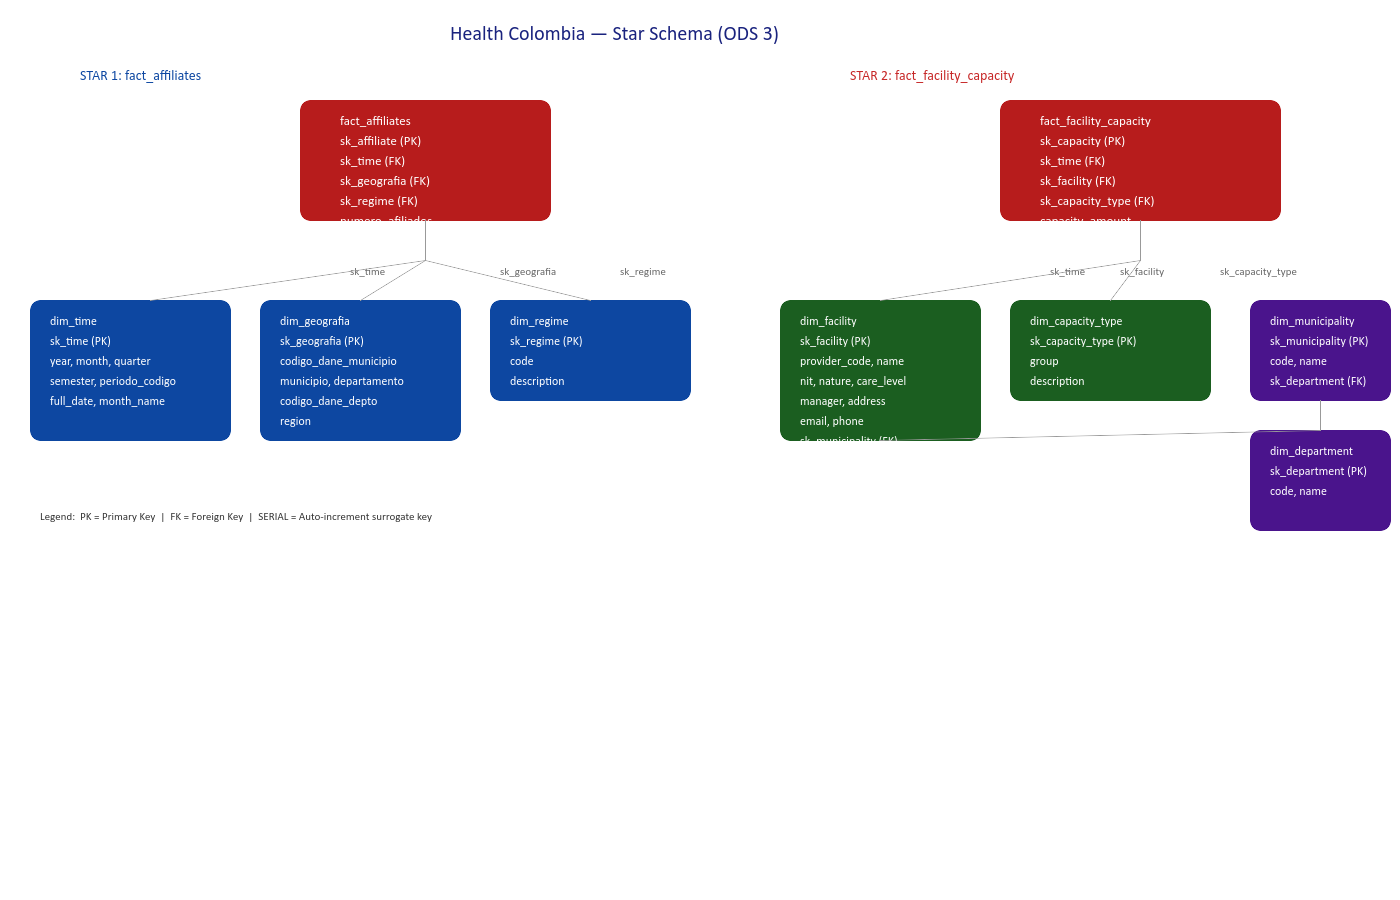
\includegraphics[width=\textwidth]{../diagrams/star_schema.png}
\caption{Star schema of the dimensional data warehouse.}
\end{figure}

\subsection{Dimension Tables}

\begin{table}[H]
\centering
\small
\begin{tabularx}{\textwidth}{p{3cm} X p{2cm}}
\toprule
\textbf{Table} & \textbf{Justification} & \textbf{Records}\\
\midrule
\texttt{dim\_time} & Temporal analysis required by R1, R2, R4, R5. Quarterly granularity. & 2\\
\addlinespace
\texttt{dim\_geografia} & Geographic analysis required by R2, R4, R5. DANE codes + region. & 2,240\\
\addlinespace
\texttt{dim\_department} & Department-level analysis required by R2, R4. Includes region. & 34\\
\addlinespace
\texttt{dim\_municipality} & Municipality granularity for territorial equity analysis (R5). & 1,168\\
\addlinespace
\texttt{dim\_regime} & Core dimension for R1, R5. Maps S/C/E/I to descriptive names. & 4\\
\addlinespace
\texttt{dim\_facility} & Facility-level analysis for R3, R4. Provider attributes. & 10,921\\
\addlinespace
\texttt{dim\_capacity\_type} & Capacity types (CAMAS/SALAS $\times$ TPR/Adultos/Pedi\'{a}trica) for R3, R4. & 63\\
\bottomrule
\end{tabularx}
\caption{Dimension tables and their analytical justification.}
\end{table}

\subsection{Fact Tables}

\begin{table}[H]
\centering
\small
\begin{tabularx}{\textwidth}{p{3.5cm} p{4cm} X p{2cm}}
\toprule
\textbf{Fact Table} & \textbf{Grain} & \textbf{Measure} & \textbf{Records}\\
\midrule
\texttt{fact\_affiliates} & Quarter + Municipality + Regime & \texttt{numero\_afiliados} & 3,369\\
\addlinespace
\texttt{fact\_facility\_capacity} & Facility + Capacity Type + Time & \texttt{capacity\_amount} & 31,496\\
\bottomrule
\end{tabularx}
\caption{Fact tables with grain and measures.}
\end{table}

\subsection{Why Two Fact Tables?}

The two fact tables have \textbf{different granularities}:
\begin{itemize}[nosep]
    \item \texttt{fact\_affiliates} is aggregated at (quarter, municipality, regime) --- a many-to-many relationship between territory and regime.
    \item \texttt{fact\_facility\_capacity} is at (facility, capacity type, time) --- individual facility-level infrastructure data.
\end{itemize}

These represent fundamentally different business processes (enrollment vs.\ infrastructure) and cannot be merged without losing analytical precision.

%%%%%%%%%%%%%%%%%%%%%%%%%%%%%%%%%%%%%%
\section{ETL Pipeline}

\subsection{Architecture}

\begin{figure}[H]
\centering
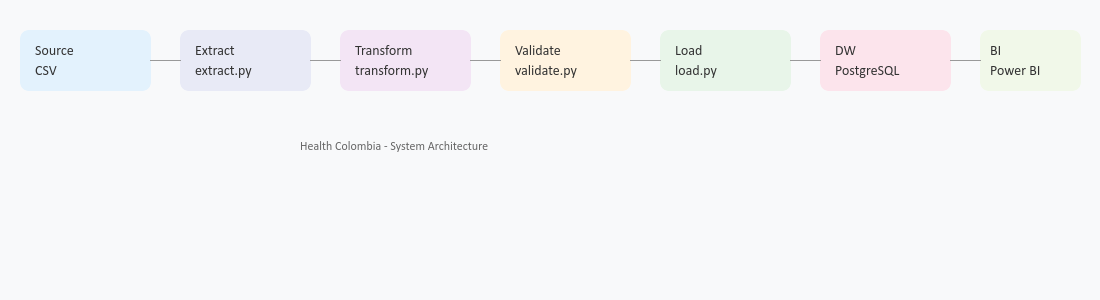
\includegraphics[width=0.9\textwidth]{../diagrams/architecture.png}
\caption{ETL pipeline architecture.}
\end{figure}

The pipeline follows a linear flow:

\begin{lstlisting}
Source CSVs -> Extract (extract.py) -> Transform (transform.py) ->
Validate (validate.py) -> Load (load.py) -> PostgreSQL DW
                                                    |
                                              CSV Export -> data/processed/
\end{lstlisting}

\subsection{Extract (\texttt{src/extract.py})}

\begin{itemize}[nosep]
    \item Reads raw CSV files with \texttt{pd.read\_csv(dtype=str)} to preserve original formatting.
    \item Renames columns from Spanish to English for consistency.
    \item Maps departments to regions using \texttt{REGION\_MAP}.
\end{itemize}

\subsection{Transform (\texttt{src/transform.py})}

\textbf{Data Preparation:}
\begin{itemize}[nosep]
    \item Removes thousand-separator periods from \texttt{NumPersonas}, converts to integer.
    \item Normalizes department and municipality names (accent removal, uppercase, alias mapping).
    \item Maps ``NO APLICA'' to ``SIN DEPARTAMENTO'' with synthetic DANE code ``00'' (preserves 1,315,701 affiliates).
    \item Maps special health districts (Cali, Cartagena, etc.) to their real departments.
    \item Extracts numeric digits from phone numbers; removes commas from NIT values.
\end{itemize}

\textbf{Dimensional Transformation:}
\begin{itemize}[nosep]
    \item Builds 7 dimension tables with surrogate keys (\texttt{sk\_*}).
    \item Generates deterministic DANE codes for facility-only municipalities using MD5 hashing.
    \item Aggregates \texttt{fact\_facility\_capacity} with \texttt{groupby().sum()} to eliminate duplicate capacity rows.
\end{itemize}

\subsection{Validate (\texttt{src/validate.py})}

\begin{table}[H]
\centering
\small
\begin{tabularx}{\textwidth}{p{3.5cm} X}
\toprule
\textbf{Rule} & \textbf{Description}\\
\midrule
FK Integrity & All foreign keys in fact tables reference existing dimension surrogate keys\\
Null Measures & No null values in \texttt{numero\_afiliados} or \texttt{capacity\_amount}\\
Negative Measures & No negative values in measure columns\\
Duplicate Keys & No duplicate composite keys in fact tables\\
Sum Consistency & Total \texttt{numero\_afiliados} matches raw CSV total within 1\% tolerance\\
Row Count & Unique facilities in fact table match source unique facilities\\
\bottomrule
\end{tabularx}
\caption{ETL validation rules.}
\end{table}

\subsection{Load (\texttt{src/load.py})}

\begin{itemize}[nosep]
    \item Connects to PostgreSQL using \texttt{psycopg2}.
    \item Executes \texttt{sql/init.sql} to reset schema (idempotent DROP + CREATE).
    \item Loads dimensions first, then fact tables, using \texttt{ON CONFLICT DO NOTHING}.
    \item Resets serial sequences after load.
    \item Single transaction: commits on success, rolls back on failure.
    \item \textbf{CSV Export:} After PostgreSQL load, exports all tables as individual CSV files to \texttt{data/processed/} for Power BI ingestion.
\end{itemize}

%%%%%%%%%%%%%%%%%%%%%%%%%%%%%%%%%%%%%%
\section{Data Quality Issues and Fixes}

During development, several critical data quality issues were identified and resolved:

\begin{table}[H]
\centering
\small
\begin{tabularx}{\textwidth}{p{4.5cm} X X}
\toprule
\textbf{Issue} & \textbf{Root Cause} & \textbf{Fix}\\
\midrule
5,072 facility rows silently dropped & Special health districts (Cali, Cartagena, Barranquilla, Santa Marta, Buenaventura) reported as ``department'' in REPS & \texttt{DISTRICT\_TO\_DEPT} mapping redirects to real departments\\
\addlinespace
80 municipalities unmapped & CAUCA missing from \texttt{DEPT\_DANE\_CODES}; facility-only municipalities not in affiliates & Added CAUCA (code 19); \texttt{build\_dim\_municipality} merges both datasets\\
\addlinespace
13,970 duplicate fact keys & Raw REPS has duplicate rows per facility + capacity type & \texttt{build\_fact\_facility\_capacity} aggregates with \texttt{groupby().sum()}\\
\addlinespace
1,315,701 affiliates lost (``NO APLICA'') & \texttt{DEPT\_NORMALIZE['NO APLICA'] = None} caused silent drop & Map to ``SIN DEPARTAMENTO'' with DANE code ``00''\\
\addlinespace
Cauca without region & CAUCA absent from \texttt{REGION\_MAP} & Added \texttt{'CAUCA': 'Pacifico'}\\
\addlinespace
Validation false positive & \texttt{len(df)} compared total rows vs unique facilities & Changed to \texttt{provider\_code.nunique()}\\
\addlinespace
Non-deterministic hash & Python \texttt{hash()} varies across runs & Replaced with \texttt{hashlib.md5()}\\
\addlinespace
Raw total computed post-clean & Validation compared against already-cleaned total & \texttt{raw\_total} computed before \texttt{clean\_affiliates()}\\
\bottomrule
\end{tabularx}
\caption{Data quality issues identified and resolved.}
\end{table}

%%%%%%%%%%%%%%%%%%%%%%%%%%%%%%%%%%%%%%
\section{Analytical Queries and KPIs}

All queries run against the PostgreSQL Data Warehouse. The complete SQL is in \texttt{sql/analytical\_queries.sql}.

\subsection{R1 --- Total Affiliates by Regime Type}

\begin{lstlisting}
SELECT r.description AS regime,
       SUM(f.numero_afiliados) AS total_affiliates,
       ROUND(SUM(f.numero_afiliados) * 100.0
             / SUM(SUM(f.numero_afiliados)) OVER(), 2) AS pct_share
FROM fact_affiliates f
JOIN dim_regime r ON f.sk_regime = r.sk_regime
GROUP BY r.description
ORDER BY total_affiliates DESC;
\end{lstlisting}

\textbf{Result:} Subsidized regime dominates with $\sim$60\% of affiliates, followed by Contributory ($\sim$38\%). Special and Individual $<$2\%.

\subsection{R2 --- Top and Bottom Departments}

Uses UNION ALL to combine the top 10 and bottom 10 departments by total affiliate count.

\textbf{Result:} Bogot\'{a} D.C., Antioquia, and Valle del Cauca concentrate the largest populations. Vaup\'{e}s, Guain\'{i}a, and Vichada have the fewest.

\subsection{R3 --- Facilities by Nature and Care Level}

\begin{lstlisting}
SELECT fc.nature, fc.care_level,
       COUNT(DISTINCT fc.sk_facility) AS facility_count,
       SUM(c.capacity_amount) AS total_capacity
FROM fact_facility_capacity c
JOIN dim_facility fc ON c.sk_facility = fc.sk_facility
GROUP BY fc.nature, fc.care_level
ORDER BY fc.nature, fc.care_level;
\end{lstlisting}

\textbf{Result:} Public facilities dominate high-complexity care (levels 3--4); private facilities concentrate in lower-complexity (levels 1--2).

\subsection{R4 --- Installed Capacity per Affiliate by Department}

Uses CTEs with FULL OUTER JOIN to combine capacity and affiliation data by department.

\textbf{Result:} Smaller departments show highly variable ratios; some have excess capacity while others face critical shortages.

\subsection{R5 --- Regime Distribution by Geographic Region}

\begin{lstlisting}
SELECT g.region, r.description AS regime,
       SUM(f.numero_afiliados) AS total_affiliates,
       ROUND(SUM(f.numero_afiliados) * 100.0
             / SUM(SUM(f.numero_afiliados))
               OVER(PARTITION BY g.region), 2) AS pct_within_region
FROM fact_affiliates f
JOIN dim_geografia g ON f.sk_geografia = g.sk_geografia
JOIN dim_regime r ON f.sk_regime = r.sk_regime
GROUP BY g.region, r.description
ORDER BY g.region, total_affiliates DESC;
\end{lstlisting}

\textbf{Result:} Andina region concentrates the majority. Subsidized affiliates are proportionally higher in Pacifico and Amazonia.

%%%%%%%%%%%%%%%%%%%%%%%%%%%%%%%%%%%%%%
\section{Validation Results}

After the full ETL pipeline execution, the following results confirm data integrity:

\subsection{Load Summary}

\begin{table}[H]
\centering
\begin{tabular}{lr}
\toprule
\textbf{Table} & \textbf{Records}\\
\midrule
dim\_time & 2\\
dim\_geografia & 2,240\\
dim\_department & 34\\
dim\_municipality & 1,168\\
dim\_regime & 4\\
dim\_facility & 10,921\\
dim\_capacity\_type & 63\\
fact\_affiliates & 3,369\\
fact\_facility\_capacity & 31,496\\
\bottomrule
\end{tabular}
\caption{Final load summary.}
\end{table}

\subsection{Data Quality Checks}

\begin{table}[H]
\centering
\begin{tabular}{ll}
\toprule
\textbf{Check} & \textbf{Result}\\
\midrule
FK nulls (fact\_affiliates) & 0\\
FK nulls (fact\_facility\_capacity) & 0\\
Negative measures & 0\\
Duplicate fact keys & 0\\
Sum consistency (affiliates) & 51,182,238 = 51,182,238 (100\% match)\\
Unmapped municipalities & 0\\
Total validation errors & \textbf{0}\\
\bottomrule
\end{tabular}
\caption{Data quality verification results.}
\end{table}

%%%%%%%%%%%%%%%%%%%%%%%%%%%%%%%%%%%%%%
\section{Business Intelligence}

A Power BI dashboard connects to the PostgreSQL Data Warehouse and provides:

\begin{itemize}[nosep]
    \item \textbf{Geographic Analysis:} Department-level map visualization showing affiliate density and capacity distribution.
    \item \textbf{Comparative Analysis:} Public vs.\ private facility distribution across care levels.
    \item \textbf{KPIs:} Total affiliates nationally, total installed capacity, capacity-to-affiliate ratio.
    \item \textbf{Filters:} By department, region, regime type, facility nature, and time period.
\end{itemize}

\textbf{Data Loading Options for Power BI:}
\begin{enumerate}[nosep]
    \item \textbf{PostgreSQL connection} (recommended): Direct connection using the PostgreSQL connector.
    \item \textbf{CSV import:} Load individual CSV files from \texttt{data/processed/} (each includes surrogate keys for joining).
\end{enumerate}

\begin{figure}[H]
\centering
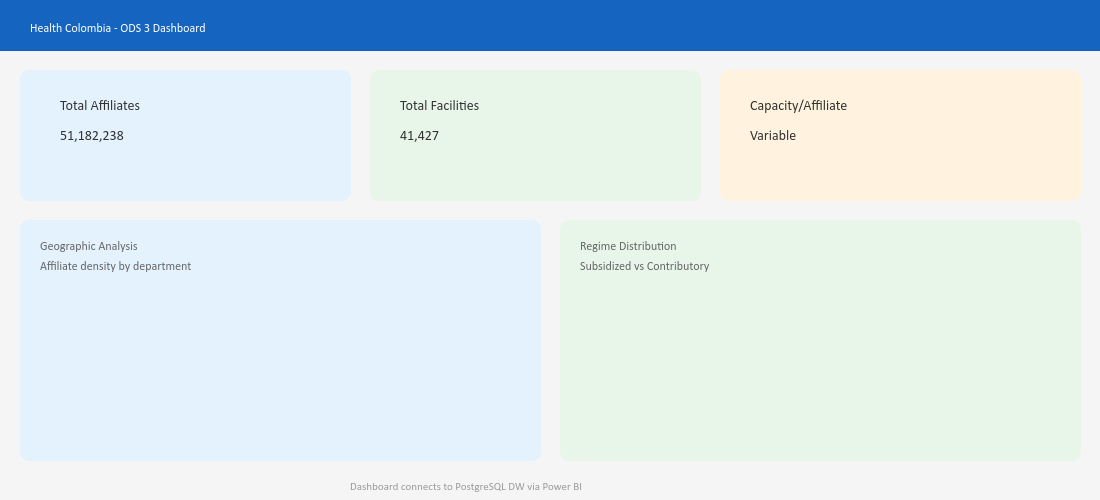
\includegraphics[width=\textwidth]{../diagrams/dashboard.png}
\caption{Power BI dashboard overview.}
\end{figure}

%%%%%%%%%%%%%%%%%%%%%%%%%%%%%%%%%%%%%%
\section{Technologies}

\begin{table}[H]
\centering
\begin{tabular}{ll}
\toprule
\textbf{Component} & \textbf{Technology}\\
\midrule
Programming & Python 3.12, Pandas, NumPy\\
Profiling & Jupyter Notebook\\
Data Warehouse & PostgreSQL 16\\
ETL Pipeline & Python (extract $\to$ transform $\to$ validate $\to$ load)\\
BI Dashboard & Power BI\\
Containerization & Docker / Podman\\
Version Control & Git, GitHub\\
Development Env & Nix Flake\\
\bottomrule
\end{tabular}
\caption{Technology stack.}
\end{table}

%%%%%%%%%%%%%%%%%%%%%%%%%%%%%%%%%%%%%%
\section{Limitations and Assumptions}

\begin{enumerate}[nosep]
    \item \textbf{Temporal snapshot:} Both datasets are cross-sectional (Q2 2022 affiliates, Q4 2022 facilities). True trend analysis requires multiple periods.
    \item \textbf{Care level gaps:} 61\% of facility records lack a care level. Missing values filled with 0 (``No reporta'').
    \item \textbf{Affiliation $\neq$ Access:} High affiliation rates do not guarantee effective healthcare access. The analysis measures enrollment, not utilization.
    \item \textbf{Capacity definition:} \texttt{capacity\_amount} represents installed capacity, not operational or effective capacity.
    \item \textbf{Cross-dataset caveat:} R4 uses Q4 2022 capacity with Q2 2022 affiliation. The ratio is indicative, not temporally precise.
    \item \textbf{Facility municipalities:} Facilities in municipalities absent from the affiliates dataset are recovered via synthetic DANE codes (MD5 hashing).
\end{enumerate}

%%%%%%%%%%%%%%%%%%%%%%%%%%%%%%%%%%%%%%
\section{Conclusions}

This project demonstrates the complete lifecycle of an ETL process applied to Colombian healthcare data:

\begin{enumerate}[nosep]
    \item \textbf{Data integration:} Two complementary datasets (SISPRO affiliates + REPS facilities) were integrated into a unified dimensional model with 7 dimension tables and 2 fact tables.
    \item \textbf{Data quality:} Eight critical data quality issues were identified and resolved, including silent data loss from special health districts, missing department codes, duplicate capacity rows, and the ``NO APLICA'' gap affecting 57\% of the Especial regime.
    \item \textbf{Analytical coverage:} All five analytical requirements (R1--R5) are fully supported by the dimensional model and verified through SQL queries.
    \item \textbf{Zero data loss:} Final validation confirms 100\% sum consistency (51,182,238 affiliates), 0 FK violations, 0 duplicate keys, and 0 negative measures.
    \item \textbf{BI readiness:} The data warehouse is accessible via PostgreSQL connection or CSV export for Power BI dashboard creation.
\end{enumerate}

The dimensional data warehouse provides a solid foundation for healthcare analytics aligned with SDG Target 3.8, enabling stakeholders to identify geographic disparities in affiliation coverage and infrastructure capacity across Colombia's territories.

%%%%%%%%%%%%%%%%%%%%%%%%%%%%%%%%%%%%%%
\section*{Team Members}

\begin{table}[H]
\centering
\begin{tabular}{p{5cm} p{3.5cm} p{5cm}}
\toprule
\textbf{Member} & \textbf{Role} & \textbf{Responsibilities}\\
\midrule
Deyton Riascos Ortiz & Project Manager & Coordinate the project, organize tasks, consolidate the final report\\
Samuel Izquierdo Bonilla & Development Team & Lead requirements definition, user stories, KPIs, data mapping\\
Daniel David Garcia Restrepo & Product Owner & Prioritize requirements, validate client needs, review business objectives\\
Mauricio Taborda Gongora & Tester & Validate data quality, verify ETL results, perform testing\\
\bottomrule
\end{tabular}
\caption{Team members and their roles.}
\end{table}

\end{document}
